\qrchapterstar{https://forgottenpillar.com/rsc/sw-fp-appendix}{Nyongeza} \label{chap:appendix}

\addcontentsline{toc}{chapter}{Nyongeza}

\section*{Kanuni za Msingi 1889}

Kama ilivyoelezwa mahali pengine, Waadventista Wasabato hawana imani ila Biblia; lakini wanashikilia mambo fulani ya imani yaliyofafanuliwa vizuri ambayo wanahisi tayari kutoa sababu “kwa kila mtu awaulizaye”. Mapendekezo yafuatayo yanaweza kuchukuliwa kama muhtasari wa sifa kuu za imani yao ya kidini, ambayo juu yake kuna, kama tujuavyo, umoja mzima katika mwili wote. Wanaoamini,—

\lettrine{I.} Kwamba kuna Mungu mmoja huluki binafsi wa kiroho, Muumba wa vitu vyote, muweza wa yote, mwenye kujua yote, na wa milele; asiye na kikomo katika hekima, utakatifu, haki, wema, ukweli, na rehema; asiyebadilika, na kila mahali akiwepo kwa mwakilishi wake, Roho Mtakatifu. Zaburi 139:7.

\lettrine{II.} Kwamba kuna Bwana mmoja Yesu Kristo, Mwana wa Baba wa Milele, ambaye kwa yeye yeye aliumba vitu vyote, na kwa yeye vinadumishwa; kwamba alichukua asili ya mbegu ya Ibrahimu kwa ukombozi wa kizazi chetu kilichoanguka; kwamba alikaa kati ya watu, amejaa neema na ukweli, aliishi kielelezo chetu, alikufa dhabihu yetu, aliinuliwa kwa ajili ya kuhesabiwa haki kwetu, alipaa juu kuwa mpatanishi wetu wa pekee katika patakatifu pa mbinguni, ambapo, kwa wema wa damu yake iliyomwagika, anapata msamaha na msamaha wa dhambi za wale wote wanaokuja kwake kwa toba; na kama sehemu ya mwisho ya kazi yake ya ukuhani, kabla hajachukua kiti chake cha enzi kama mfalme, yeye atafanya upatanisho mkubwa kwa dhambi za wote hao, na dhambi zao zitafutwa (Matendo 3:19) na kuchukuliwa mbali na patakatifu, kama inavyoonyeshwa katika utumishi wa ukuhani wa Walawi, ambao ulitangulia na kufananisha huduma ya Bwana wetu aliye mbinguni. Tazama Mambo ya Walawi 16; Waebrania 8:4, 5; 9:6, 7; na kadhalika.

\lettrine{III.} Kwamba Maandiko Matakatifu ya Agano la Kale na Agano Jipya yalitolewa kwa uvuvio wa Mungu, yana ufunuo kamili ya mapenzi yake kwa mwanadamu, na ndiyo kanuni pekee isiyoweza kukosea ya imani na mazoezi.

\lettrine{IV.} Kwamba Ubatizo ni agizo la kanisa la Kikristo, kufuata imani na toba—agizo ambalo kwalo tunaadhimisha ufufuo wa Kristo, kwani kwa tendo hili tunaonyesha Imani yetu katika kuzikwa na kufufuka kwake, na kwa njia hiyo, katika ufufuo wa watakatifu wote katika ufufuo siku ya mwisho; na kwamba hakuna hali nyingine inayowakilisha ukweli huu kwa ufaafu zaidi ya ile ambayo Maandiko yanaagiza, yaani, kuzamishwa. Warumi 6:3-5; Wakolosai 2:12.

\lettrine{V.} Kwamba kuzaliwa upya kunajumuisha mabadiliko yote muhimu ili kutufaa kwa ufalme wa Mungu; na lina sehemu mbili; Kwanza, mabadiliko ya kimaadili yanayoletwa na wongofu na maisha ya Kikristo (Yohana 3:3, 5); pili, mabadiliko ya kimwili katika ujio wa pili wa Kristo, ambapo, ikiwa tumekufa, tunafufuliwa bila kuharibika, na ikiwa tunaishi, tunabadilishwa kuwa kutokufa kwa dakika moja, ndani kufumba na kufumbua. Luka 20:36; 1 Wakorintho 15:51, 52.

\lettrine{VI.} Kwamba Unabii ni sehemu ya ufunuo wa Mungu kwa mwanadamu; kwamba imejumuishwa katika Maandiko hayo ambayo yafaa kwa mafundisho (2 Timotheo 3:16); kwamba imeundwa kwa ajili yetu na watoto wetu (Kumbukumbu la Torati 29:29); kwamba mbali na kugubikwa na fumbo lisilopenyeka, ni hilo ambayo hasa hufanya neno la Mungu kuwa taa ya miguu yetu na mwanga wa njia yetu (Zaburi 119:105; 2 Petro 1:19); kwamba baraka inatamkwa juu ya wale wanaoisoma (Ufunuo 1:1-3); na kwamba, kwa hivyo, inapaswa kueleweka na watu wa Mungu vya kutosha kuwaonyesha msimamo wao katika historia ya ulimwengu na majukumu maalum yanayohitajika mikononi mwao.

\lettrine{VII.} Kwamba historia ya dunia kutoka tarehe maalum katika siku za nyuma, kupanda na kuanguka kwa himaya, na mfululizo wa matukio hadi kusimamishwa kwa ufalme wa milele wa Mungu, yameainishwa katika minyororo mingi mikuu ya unabii; na kwamba unabii huu wote sasa umetimia isipokuwa matukio ya kufunga.

\lettrine{VIII.} Kwamba fundisho la uongofu wa ulimwengu na milenia ya muda ni hekaya ya siku hizi za mwisho, zilizohesabiwa kuwarubuni watu katika hali ya usalama wa kimwili, na kuwafanya kupatikana na siku ile kuu ya Bwana kama vile mwivi usiku (1 Wathesalonike 5:3); hiyo ujio wa pili wa Kristo ni kutangulia, si kufuata, milenia; kwa maana mpaka Bwana aonekane, mamlaka ya upapa, pamoja na machukizo yake yote, yataendelea (2 Wathesalonike 2:8), ngano na magugu hukua pamoja (Mathayo 13:29, 30, 39), na watu waovu na wadanganyi huzidi kuwa mbaya zaidi na mbaya zaidi, kama neno la Mungu linavyotangaza. 2 Timotheo 3:1, 13.

\lettrine{IX.} Kwamba kosa la Waadventista mwaka 1844 lilihusu asili ya tukio basi kwa kutokea, si kwa wakati; kwamba hakuna kipindi cha kinabii kinachotolewa kufikia ujio wa pili, bali kwamba ile ndefu zaidi, zile siku elfu mbili na mia tatu za Danieli 8:14, ziliisha 1844, na kutuleta kwenye tukio linaloitwa utakaso wa patakatifu.

\lettrine{X.} Kwamba patakatifu pa agano jipya ni maskani ya Mungu mbinguni, ambayo Paulo hunena katika Waebrania 8 na kuendelea, na ambayo Bwana wetu, aliye kuhani mkuu, anahudumu; kwamba patakatifu hapa ni mfano wa hema ya Musa, na kwamba kazi ya ukuhani wa Bwana wetu, aliyeunganishwa nayo, ndiye mfano wa kazi ya makuhani wa Kiyahudi wa kipindi cha zamani (Waebrania 8:1-5, nk.); kwamba hii, na si dunia, ni patakatifu pa kutakaswa mwishoni mwa zile siku elfu mbili na mia tatu, zile zinazoitwa utakaso zake kuwa katika kesi hii, kama mfano, kuingia tu kwa kuhani mkuu katika mahali patakatifu pa patakatifu, ili kumalizia duru ya huduma iliyounganishwa nayo, kwa kufanya upatanisho na kuondoa kutoka kwa Patakatifu dhambi zilizohamishwa kwake kwa njia ya huduma katika chumba cha kwanza (Mambo ya Walawi 16; Waebrania 9:22, 23); na kwamba kazi hii katika mfano, kuanzia 1844, inajumuisha kufuta dhambi za waumini (Matendo 3:19), na inachukua muda mfupi lakini usio na kipimo wa wakati, katika hitimisho ambalo kazi ya rehema kwa ulimwengu itakamilika, na ujio wa pili wa Kristo utatokea.

\lettrine{XI.} Kwamba matakwa ya Mungu ya kimaadili ni sawa kwa wanadamu wote katika vipindi vyote; Kwamba haya yamo katika amri zilizonenwa na Yehova kutoka Sinai, zilizochongwa juu ya mbao za mawe, na kuwekwa katika safina, ambayo ilikuwa katika matokeo iliitwa “sanduku la agano,” au agano (Hesabu 10:33; Waebrania 9:4, nk.); kwamba sheria hii isiyobadilika na ya kudumu, ikiwa ni nakala ya meza zilizowekwa ndani ya safina katika patakatifu pa kweli palipo juu, ambapo pia, kwa sababu iyo hiyo, huitwa sanduku la agano la Mungu; wakati wa kupigwa kwa baragumu ya saba tunaambiwa kwamba “hekalu la Mungu likafunguliwa mbinguni, na sanduku la agano lake lilionekana katika hekalu lake.” Ufunuo 11:19.

\lettrine{XII.} Kwamba amri ya nne ya sheria hii inatutaka tuiweke siku ya saba ya kila juma, inayojulikana sana kuwa Jumamosi, kujiepusha na kazi yetu wenyewe, na kwa utekelezaji wa majukumu matakatifu na ya kidini; kwamba hii ndiyo Sabato pekee ya kila juma inayojulikana kwa Biblia, ikiwa ni siku iliyotengwa kabla ya Paradiso kupotea (Mwanzo 2:2, 3), na ambayo itaadhimishwa katika Paradiso iliyorudishwa (Isaya 66:22, 23); kwamba ukweli kuhusu Maadhimisho ya Sabato ni msingi wa kuifungia siku ya saba, kwa kuwa si kweli kwa siku yoyote nyingine; na kwamba maneno Sabato ya Kiyahudi, kama inavyotumika kwa siku ya saba, na Sabato ya Mkristo, kama inavyotumiwa kwa siku ya kwanza ya juma, ni majina ya uvumbuzi wa wanadamu, yasiyo ya kimaandiko kwa kweli, na maana ya uwongo.

\lettrine{XIII.} Kwamba kama mtu wa dhambi, upapa, amefikiria kubadili nyakati na sheria (sheria ya Mungu, Danieli 7:25), na amepotosha karibu Jumuiya ya Wakristo yote kuhusiana na ile amri ya nne, tunapata unabii wa mageuzi katika suala hili kufanywa kati ya waumini kabla tu ya kuja kwa Kristo. Isaya 56:1, 2; 1 Petro 1:5; Ufunuo 14:12, nk.

\lettrine{XIV.} Kwamba wafuasi wa Kristo wanapaswa kuwa watu wa kipekee, si kufuata kanuni wala wakipatana na njia za ulimwengu; kutopenda anasa zake wala kukabili upumbavu wake; kama vile mtume asemavyo kwamba “yeyote atakaye kuwa” katika maana hii, “rafiki wa ulimwengu ni adui wa Mungu” (Yakobo 4:4); na Kristo anasema kwamba hatuwezi kuwa na mabwana wawili, au, wakati huo huo, kumtumikia Mungu na mali. Mathayo 6:24.

\lettrine{XV.} Kwamba Maandiko yanasisitiza juu ya uwazi na staha ya mavazi kama alama kuu ya ufuasi kati ya wale wanaodai kuwa wafuasi wa Yeye ambaye alikuwa, “mpole na mnyenyekevu katika moyo,” kwamba kuvaa dhahabu, lulu, na mavazi ya bei ghali, au chochote kilichobuniwa tu kupamba mtu na kukuza kiburi cha moyo wa asili, ni kutupwa, kulingana na maandiko kama vile 1 Timotheo 2:9, 10; 1 Petro 3:3, 4.

\lettrine{XVI.} Kwamba rasilimali kwa ajili ya msaada wa kazi ya kiinjilisti kati ya watu inapaswa kuchangiwa kwa upendo kwa Mungu na upendo wa roho, sio kukuzwa na bahati nasibu ya kanisa, au hafla zilizokusudiwa kuchangia tabia ya kupenda kujifurahisha, na kufurahisha tamaa ya mwenye dhambi, kama vile maonyesho, sherehe, karamu za oyster, chai, ufagio, punda, na jamii za wazimu, n.k., ambazo ni aibu kwa kanisa linalojiita la Kristo; kwamba sehemu ya mapato ya mtu inayohitajika hapo awali maongozi hayawezi kuwa machache chini ya injili; kwamba ni sawa na Ibrahimu (ambaye sisi ni watoto, kama sisi ni wa Kristo, Wagalatia 3:29) tunalipwa kwa Melkizedeki (aina ya Kristo) wakati alimpa sehemu ya kumi ya vitu vyote (Waebrania 7:1-4); cheo ni cha Bwana (Mambo ya Walawi 27:30); na hii sehemu ya kumi ya mapato ya mtu pia inapaswa kuongezwa na matoleo kutoka kwa wale wanaoweza, kwa msaada wa injili. 2 Wakorintho 9:6; Malaki 3:8, 10.

\lettrine{XVII.} Kwamba kama vile moyo wa asili au wa kimwili uko katika uadui na Mungu na sheria yake, uadui huu unaweza kutiishwa tu na mabadiliko makubwa ya mapenzi, kubadilishana kanuni yasiyo takatifu kwa matakatifu; kwamba mageuzi haya yanafuata toba na imani, ni kazi maalum ya Roho Mtakatifu, na hujumuisha kuzaliwa upya, au kuongoka.

\lettrine{XVIII.} Kwamba kama wote wamevunja sheria ya Mungu, na hawawezi kwa wao wenyewe kutoa utii kwa matakwa yake ya haki, tunamtegemea Kristo, kwanza, kwa ajili ya kuhesabiwa haki kutokana na makosa yetu ya zamani, na pili, kwa neema ambayo kwayo wanaweza kutoa utii unaokubalika kwa sheria yake takatifu katika wakati ujao.

\lettrine{XIX.} Kwamba Roho wa Mungu aliahidiwa kujidhihirisha ndani ya kanisa kupitia karama Fulani, imeorodheshwa hasa katika 1 Wakorintho 12 na Waefeso 4; kwamba karama hizi sio iliyokusudiwa kuchukua nafasi, au kuchukua mahali pa, Biblia, ambayo inatosha kutufanya tuwe na hekima kwa wokovu, kama vile Biblia haiwezi kuchukua mahali pa Roho Mtakatifu; hivyo, katika kibainisha mikondo mbalimbali ya utendaji wake, Roho huyo ameifanya kwa urahisi uwepo na uwepo wake pamoja na watu wa Mungu hadi mwisho wa nyakati, ili kuongoza kwenye ufahamu wa neno lile ambalo lilikuwa limevuviwa, kusadikisha juu ya dhambi, na kufanya kazi ya mabadiliko katika moyo na maisha; na kwamba wale wanaomkana Roho mahali pake na utendakazi wake, hukataa kwa uwazi ile sehemu ya Biblia ambayo inaipa kazi hii na msimamo huu.

\lettrine{XX.} Kwamba Mungu, kwa mujibu wa shughuli zake sawa na wanadamu, anatuma tangazo la kukaribia kwa ujio wa pili wa Kristo; na kwamba kazi hii inafananishwa na jumbe tatu za Ufunuo 14, ujumbe wa mwisho unaoleta kutazama kazi ya kurekebisha sheria ya Mungu, ili watu wake wapate kuwa tayari kabisa kwa ajili ya tukio hilo.

\lettrine{XXI.} Kwamba wakati wa kutakaswa kwa patakatifu (Angalia pendekezo la X.), linalolingana na wakati wa kutangazwa kwa ujumbe wa tatu (Ufunuo 14:9, 10), ni wakati wa hukumu ya uchunguzi, kwanza, kwa kuzingatia wafu, na pili, mwishoni mwa muda wa majaribio, kwa kurejelea walio hai, ili kubaini ni nani kati ya maelfu ya maelfu ya watu wanaolala ndani ya mavumbi ya nchi wanastahili sehemu katika ufufuo wa kwanza, na ni nani kati ya watu wake walio hai wanastahili kubadilishwa,—mambo ambayo ni lazima yaamuliwe kabla ya Bwana kutokea.

\lettrine{XXII.} Kwamba kaburi, ambao sisi sote tunaelekea, linaonyeshwa na neno la Kiebrania sheol na Neno la Kigiriki hades, ni mahali, au hali, ambapo hakuna kazi, kifaa, hekima, wala maarifa. Mhubiri 9:10.

\lettrine{XXIII.} Kwamba hali ambayo tunapunguzwa na kifo ni ya ukimya, kutofanya kazi, na kupoteza fahamu. Zaburi 146:4; Mhubiri 9:5, 6; Danieli 12:2.

\lettrine{XXIV.} Kwamba kutoka katika gereza hili la kaburi, wanadamu wataletwa kwa ufufuo wa mwili; wenye haki walio na sehemu katika ufufuo wa kwanza, utakaofanyika katika ujio wa pili wa Kristo; waovu, katika ufufuo wa pili, unaofanyika katika miaka elfu baada ya hapo. Ufunuo 20:4-6.

\lettrine{XXV.} Kwamba wakati wa parapanda ya mwisho, wenye haki walio hai watabadilishwa mara moja, katika kupepesa macho, na wenye haki waliofufuka watanyakuliwa ili kumlaki Bwana katika anga, hivyo kuwa na Bwana milele. 1 Wathesalonike 4:16, 17; 1 Wakorintho 15:51, 52.

\lettrine{XXVI.} Kwamba hawa wasioweza kufa kisha wanachukuliwa kwenda mbinguni, kwenye Yerusalemu Mpya, Nyumba ya Baba, ambamo mna makao mengi (Yohana 14:1-3), ambamo wanatawala naye Kristo miaka elfu, wakihukumu ulimwengu na malaika walioanguka, yaani, kugawanya adhabu itakayotekelezwa juu yao mwishoni mwa ile miaka elfu moja (Ufunuo 20:4; 1 Wakorintho 6:2, 3); kwamba wakati huu dunia iko katika ukiwa na hali ya machafuko (Yeremia 4:23-27), iliyofafanuliwa, kama hapo mwanzo, na neno la Kiyunani abussos— “shimo lisilo chini” (Septuagint ya Mwanzo 1:2); na kwamba hapa Shetani amefungwa wakati wa miaka elfu (Ufunuo 20:1, 2) na hapa hatimaye kuharibiwa (Ufunuo 20:10; Malaki 4:1); ukumbi wa michezo wa uharibifu alioufanya katika ulimwengu ukifanywa ipasavyo, kwa wakati, jela yake yenye huzuni, na kisha mahali pa uangamizaji wake kwa mwisho.

\lettrine{XXVII.} Kwamba mwisho wa ile miaka elfu Bwana atashuka pamoja na watu wake na Yerusalemu Mpya (Ufunuo 21:2), wafu waovu wanafufuliwa, na wanakuja juu ya uso wa dunia nchi isiyofanywa upya, na kuuzunguka mji, kambi ya watakatifu (Ufunuo 20:9), na moto unashuka kutoka mbinguni kwa Mungu na kuwateketeza. Kisha huliwa, mzizi na tawi (Malaki 4:1) na kuwa kana kwamba hawakuwapo. Obadia 15, 16. Katika uharibifu huu wa milele kutoka kwa uwepo wa Bwana (2 Wathesalonike 1:9), waovu wanakutana na “adhabu ya milele” iliyotishwa dhidi yao (Mathayo 25:46), ambayo ni kifo cha milele. Warumi 6:23; Ufunuo 20:14, 15. Huku ndiko kuangamia kwa watu wasiomcha Mungu; moto unaowateketeza ukiwa ni moto ambao kwa ajili yake “mbingu na nchi ziko sasa,... zimehifadhiwa.” ambayo itayeyusha hata vitu vya asili kwa ukali wake, na kuvisafisha ardhi kutoka kwenye madoa ya ndani kabisa ya laana ya dhambi. 2 Petro 3:7-12.

\lettrine{XXVIII.} Kwamba mbingu mpya na nchi mpya zitachipuka kwa uwezo wa Mungu kutoka majivuni ya kale, na dunia hii iliyofanywa upya, pamoja na Yerusalemu Mpya kwa ajili ya jiji lake kuu na mji mkuu wake, patakuwa urithi wa milele wa watakatifu, mahali ambapo wenye haki watakaa milele. 2 Petro 3:13; Zaburi 37:11, 29; Mathayo 5:5.

\section*{Kanuni za Kimsingi - Msururo wa Wakati} \label{appendix:timeline}

Ifuatayo ni orodha ya baadhi ya matokeo ya Tangazo la Kanuni za Kimsingi katika machapisho yetu. Viungo vyote vinapatikana katika \href{https://notefp.link/fp-timeline}{https://notefp.link/fp-timeline}.

\leftsubsection{1872 - Matokeo ya kwanza}

\textit{“A Declaration of the Fundamental Principles, Taught and Practiced by the Seventh-Day Adventists”} - ilichapishwa kama kijitabu (\href{https://adventistdigitallibrary.org/islandora/object/adl:366607?link_only=true}{skani ya asili} \href{https://forgotten-pillar.s3.us-east-2.amazonaws.com/A+declaration+of+the+fundamental+principles+taught+and+practiced+by+the+Seventh-day+Adventists++.pdf}{*}). Zilionekana bila jina, zikiwasilishwa kama muhtasari mfupi wa umma wa kile Waadventista Wasabato wanaamini.

\leftsubsection{1874 - The Signs of the Times}

Skani ya asili: \href{https://adventistdigitallibrary.org/adl-364148/signs-times-june-4-1874}{ST Juni 4, 1874, uk.3.} \href{https://forgotten-pillar.s3.us-east-2.amazonaws.com/Signs+of+the+Times+_+June+4%2C+1874++.pdf}{*} James White alisimama nyuma ya tangazo kama mhariri mkuu wa Signs of the Times wakati huo.

\leftsubsection{1874 - The Advent Review and Herald of the Sabbath}

Skani ya asili: \href{https://documents.adventistarchives.org/Periodicals/RH/RH18741124-V44-22.pdf}{RH Novemba 24, 1874, uk.171} \href{https://forgotten-pillar.s3.us-east-2.amazonaws.com/RH18741124-V44-22.pdf}{*} Uriah Smith alitia saini tangazo kama mhariri mkuu wa Review and Herald of the Sabbath wakati huo.

\leftsubsection{1874 - Part of a booklet: The Seventh-day Adventists: A Brief Sketch of Their Origin, Progress, and Principles}

Kijitabu kilichapishwa tena mwaka 1876 na 1878 na miaka ya baadaye. \\
Nakala ya asili: (\href{https://adventistdigitallibrary.org/islandora/object/adl%3A22250872?solr_nav%5Bid%5D=a09d3902c2540c98eb7f&solr_nav%5Bpage%5D=56&solr_nav%5Boffset%5D=3}{nakala ya 1878})

\leftsubsection{1875 - The Signs of the Times}

Nakala ya asili: \href{https://documents.adventistarchives.org/Periodicals/ST/ST18750128-V01-14.pdf#search=ST18750128}{ST Januari 28, 1875} \href{https://forgotten-pillar.s3.us-east-2.amazonaws.com/ST18750128-V01-14.pdf}{*} (uk. 108, 109)

\leftsubsection{1878 - The Signs of the Times}

Nakala ya asili: \href{https://documents.adventistarchives.org/Periodicals/ST/ST18780221-V04-08.pdf#search=%22As%20already%20stated%2C%20S%2E%20D%2E%20Adventists%22}{ST Februari 21, 1878} \href{https://forgotten-pillar.s3.us-east-2.amazonaws.com/ST18780221-V04-08.pdf}{*} (uk. 59)

\leftsubsection{1888 - Gospel Sickle, April 1, 1888}

Nakala ya asili: \href{https://adventistdigitallibrary.org/adl-410336/gospel-sickle-april-1-1888?view_only=true&solr_nav%5Bid%5D=ff4d7f3f77b9bdf9e9ac&solr_nav%5Bpage%5D=0&solr_nav%5Boffset%5D=6}{Gospel Sickle, Aprili 1, 1888}

\leftsubsection{1888 - The Present Truth, August 16, 1888}

Nakala ya asili: \href{https://adventistdigitallibrary.org/adl-402854/present-truth-august-16-1888?view_only=true&solr_nav%5Bid%5D=ff4d7f3f77b9bdf9e9ac&solr_nav%5Bpage%5D=0&solr_nav%5Boffset%5D=13}{PT18880816} (uk. 250 - 252)

\leftsubsection{1889 - SDA Yearbook for 1889}

Skani asilia: \href{https://documents.adventistarchives.org/Yearbooks/YB1889.pdf#search=Yearbook%201889}{YB1889} \href{https://forgotten-pillar.s3.us-east-2.amazonaws.com/YB1889.pdf}{*} (uk. 145 - 151) Uriah Smith alipanua Kanuni za Msingi hadi mapendekezo 28. Aliongeza nukta kuhusu utakaso (nukta 14), mageuzi ya mavazi (nukta 15) na zaka (nukta 16). Pia alifanya mabadiliko madogo ya kimaandishi katika baadhi ya maelezo, lakini maana ilibaki sawa.

\leftsubsection{1897 - Words of Truth - no. 5}

Skani asilia: \href{https://adl.b2.adventistdigitallibrary.org/concern/published_works/4ffda25e-a06b-48d4-8ace-67cdcd33726f}{WoT no.5}
Word of Truth ilikuwa mfululizo wa vijitabu vyenye \href{https://adl.b2.adventistdigitallibrary.org/concern/parent/22267078_fundamental_principles_of_seventh_day_adventists/published_works/94a22141-33e8-4b9a-b397-2fe48c17bec4}{sehemu 29}.

\leftsubsection{1905 - SDA Yearbook for 1905}

Skani asilia: \href{https://documents.adventistarchives.org/Yearbooks/YB1905.pdf#search=Yearbook%201905}{YB1905} \href{https://forgotten-pillar.s3.us-east-2.amazonaws.com/YB1905.pdf}{*} (uk. 188 - 192)

\leftsubsection{1907 - SDA Yearbook for 1907}

Skani asilia: \href{https://documents.adventistarchives.org/Yearbooks/YB1907.pdf#search=Yearbook%201906}{YB1907} \href{https://forgotten-pillar.s3.us-east-2.amazonaws.com/YB1907.pdf}{*} (uk. 175 - 179)

\leftsubsection{1908 - SDA Yearbook for 1908}

Skani asilia: \href{https://documents.adventistarchives.org/Yearbooks/YB1908.pdf#search=Yearbook%201906}{YB1908} \href{https://forgotten-pillar.s3.us-east-2.amazonaws.com/YB1908.pdf}{*} (uk. 213 - 217)

\leftsubsection{1909 - SDA Yearbook for 1909}

Skani ya asili: \href{https://documents.adventistarchives.org/Yearbooks/YB1909.pdf#search=Yearbook%201909}{YB1909} \href{https://forgotten-pillar.s3.us-east-2.amazonaws.com/YB1909.pdf}{*} (uk. 220 - 224)

\leftsubsection{1910 - SDA Yearbook for 1910}

Skani ya asili: \href{https://documents.adventistarchives.org/Yearbooks/YB1910.pdf#search=Yearbook%201910}{YB1910} \textbf{\href{https://forgotten-pillar.s3.us-east-2.amazonaws.com/YB1910.pdf}{*}} (uk. 224 - 228)

\leftsubsection{1911 - SDA Yearbook for 1911}

Skani ya asili: \href{https://documents.adventistarchives.org/Yearbooks/YB1911.pdf#search=Yearbook%201910}{YB1911} \href{https://forgotten-pillar.s3.us-east-2.amazonaws.com/YB1911.pdf}{*} (uk. 223 - 227)

\leftsubsection{1912 - Advent Review and Sabbath Herald, August 22, 1912}

Skani ya asili: \href{https://adventistdigitallibrary.org/adl-351682/advent-review-and-sabbath-herald-august-22-1912?view_only=true&solr_nav%5Bid%5D=ff4d7f3f77b9bdf9e9ac&solr_nav%5Bpage%5D=0&solr_nav%5Boffset%5D=15}{RH19120822} (uk. 4 - 6)

\leftsubsection{1912 - SDA Yearbook for 1912}

Skani ya asili: \href{https://documents.adventistarchives.org/Yearbooks/YB1912.pdf#search=Yearbook%201910}{YB1912} \href{https://forgotten-pillar.s3.us-east-2.amazonaws.com/YB1912.pdf}{*} (uk. 261 - 265)

\leftsubsection{1913 - SDA Yearbook for 1913}

Skani ya asili: \href{https://documents.adventistarchives.org/Yearbooks/YB1913.pdf#search=Yearbook%201913}{YB1913} \href{https://forgotten-pillar.s3.us-east-2.amazonaws.com/YB1913.pdf}{*} (uk. 281 -285 )

\leftsubsection{1914 - SDA Yearbook for 1914}
Skani ya asili: \href{https://documents.adventistarchives.org/Yearbooks/YB1914.pdf#search=Yearbook%201914}{YB1914} \href{https://forgotten-pillar.s3.us-east-2.amazonaws.com/YB1914.pdf}{*} (uk. 293 - 297)

\section*{Ripoti ambazo hazijathibitishwa katika maandishi ya Ellen White}

\label{appendix:unauthenticated-reports}
Tungependa kuwasilisha kwako nukuu moja ya Ellen White ambayo inapinga hitimisho la umbile la Roho Mtakatifu. Katika somo hili, tumeona kwamba Roho Mtakatifu ni roho na si kiumbe. Katika kujifunza \emcap{umbile la Mungu} na mahali uwepo wake ulipo, tumeona tofauti kati ya maneno ‘kiumbe’ na ‘roho’. Tulifikia hitimisho kwamba Baba na Mwana ni viumbe wawili tofauti, kwa hivyo wamebanwa angani, wakati Roho Mtakatifu ni roho, njia ambayo Baba na Mwana wanapatikana kila mahali.

Nukuu ifuatayo inashuhudia kwamba Roho Mtakatifu pia ni kiumbe, kama vile Baba na Mwana ni viumbe:

\egw{Hapa ndipo kazi ya Roho Mtakatifu inapoingia, baada ya ubatizo wako. Unabatizwa katika jina la \textbf{Baba, la Mwana, na la Roho Mtakatifu}. Umeinuliwa nje ya maji kuishi tangu sasa katika upya wa maisha—kuishi maisha mapya. Umezaliwa kwa Mungu, na unasimama chini ya kibali na \textbf{uwezo wa \underline{viumbe} watatu watakatifu zaidi mbinguni}, ambao wanaweza kukuzuia usianguke.}[Ms95-1906.29; 1906][https://egwwritings.org/read?panels=p8872.35]

Wengi wamekutana na nukuu hii na kuiwasilisha kama uthibitisho kwamba Roho Mtakatifu ni kiumbe badala ya roho. Ifuatayo, tunawasilisha wasiwasi wetu.

Chanzo cha nukuu hii ni Hati ya 95, 1906.

Nukuu hii kwa hakika ni ripoti kutoka kwa mahubiri ya Dada White yaliyofanyika Oakland, California, siku ya Sabato alasiri, Oktoba 20, 1906. Mengi ya mahubiri ya hadhara ya Ellen White yalikuwa yakiripotiwa kwa maandishi na baadaye kuandikwa upya ili kuchapishwa. Dada White alipohubiri, hakuwahi kuwa na mahubiri yaliyoandikwa. Hakukuwa na vinasa sauti wakati huo ambavyo vingeweza kuandika kwa usahihi neno kwa neno. Rejea pekee tuliyo nayo kutoka wakati huo ni ripoti ya stenografa. Hii inafungua uwezekano wa makosa ya kibinadamu katika kuripoti, au kuhariri baadaye, kabla ya kuchapishwa. Wingi wa ushahidi uliotolewa katika kitabu hiki unaweka wazi kwamba taarifa hii haipatani na nukuu zilizothibitishwa. Imesemwa wazi, ni dhahiri kwamba kosa lilifanywa katika ripoti ya mahubiri haya.

Ili kuondoa makosa kama hayo kwa vizazi vijavyo, Dada White anatuonya inapofikia ripoti ambazo hazijaidhinishwa za kile ambacho anaweza kuwa alisema.

\egw{Na sasa kwa wote ambao wana hamu ya ukweli ningesema: \textbf{Usikubali ripoti ambazo hazijathibitishwa kuhusu kile Dada White amefanya au kusema au kuandika}. Ikiwa una hamu ya kujua yale ambayo Bwana amefunua kupitia kwake, \textbf{soma kazi zake zilizochapishwa}. Je! kuna mambo yoyote ya kuvutia ambayo hajaandika, usipate kwa shauku na kuripoti uvumi kuhusu alichosema.}[5T 696.1; 1889][https://egwwritings.org/read?panels=p113.3386]

Kazi zilizochapishwa za Ellen White wakati wa maisha yake zinawakilisha sahihi na ni maandishi ya kweli kutoka kwa Dada White. Mchakato wa uchapishaji ulihakikisha kuwa bidhaa ya mwisho ilikuwa halisi. Uzito wa ushahidi ni kwamba Dada White mwenyewe alihusika katika mchakato huo ya uchapishaji na angekagua miswada kabla ya kuchapishwa.

\egw{Nilisoma juu ya yote yaliyonakiliwa, ili kuona kwamba kila kitu ni kama inavyopaswa kuwa. Nilisoma maandishi yote ya kitabu kabla ya kutumwa kwa kichapishi.}[Lt133-1902.4; 1902][https://egwwritings.org/read?panels=p9791.10]

\egw{Nimechunguza vichapo vyangu vyote kwa karibu. Natamani kwamba hakuna kitu kitakachoonekana kwa kuchapishwa bila uchunguzi wa kina.}[Lt49-1894.11; 1894][https://egwwritings.org/read?panels=p5289.20]

Taarifa kwamba Roho Mtakatifu ni nafsi haikuwa sehemu ya mchakato wa uchapishaji kwa sababu taarifa hii ilionekana baada ya kifo cha Ellen White. Kwa hivyo, haijathibitishwa. Si mali ya “kazi yake iliyochapishwa”. Hatutafuti njama yoyote katika hili; sisi ni kwa kuzingatia tu pendekezo la Ellen White la kutokubali ripoti hizi. Katika 1990, Ellen White Estate ilichapisha mkusanyiko wa mahubiri na mazungumzo yake na mnamo 2015, ilijumuisha mahubiri na mazungumzo katika mafaili ya Maandishi yake. Hatuelewi kwa nini walifanya hivyo kwa vile mahubiri na mazungumzo hayana maandishi kutoka kwa Ellen White, lakini kutoka kwa baadhi ya waandishi wa stenograph. Walakini, juu ya kila hati ya EGW Estate ilibainisha chanzo chake, iwe ni mahubiri au barua. Hii inatuambia ikiwa nukuu imethibitishwa au la.

\begin{figure}
    \centering
    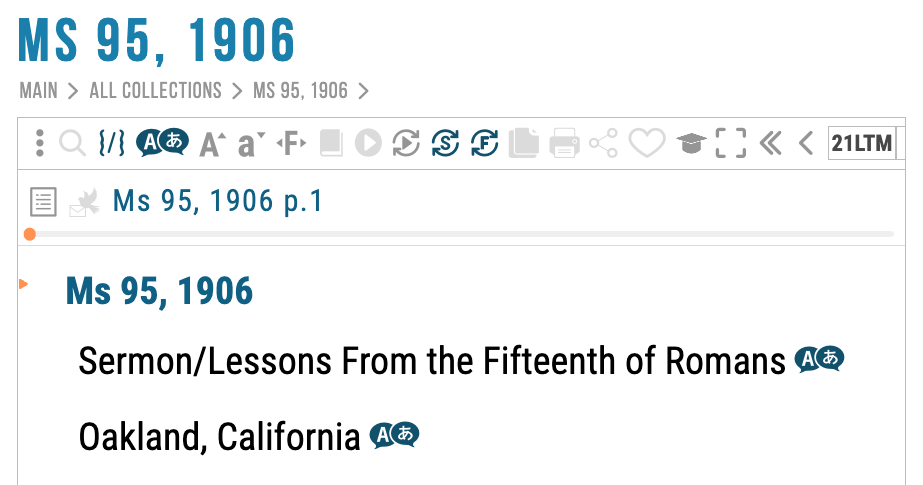
\includegraphics[width=1\linewidth]{images/sermons-and-talks.png}
    \label{fig:enter-label}
\end{figure}

Kwa sisi, kibinafsi, nukuu hizi hazijathibitishwa na, haswa, ni batili ikilinganishwa na Kazi zilizothibitishwa za Ellen White. Lakini ikiwa mtu anasisitiza kumpima bila kuthibitishwa kwa ripoti na maandishi yaliyochapishwa kwa usawa, hatutasimama katika njia yao lakini hata kusukuma zaidi hitimisho la Roho Mtakatifu kama kiumbe. Tufuate pamoja.

Hata ikilinganishwa na kazi zilizothibitishwa za Ellen White, hiyo Roho Mtakatifu kama, kiumbe, angefanya isiwe kitu kimoja na Mungu kwa sababu Kristo alikuwa \egwinline{\textbf{Nafsi pekee ambaye alikuwa mmoja na Mungu}}[Lt121-1897.7; 1897][https://egwwritings.org/read?panels=p7266.13]. Huyu Roho Mtakatifu, kama nafsi, hakuweza \egwinline{\textbf{kuingia katika mashauri na makusudi yote ya Mungu}}, kwa sababu Kristo alikuwa \egwinline{\textbf{Nafsi pekee}}[PP 34.1; 1890][https://egwwritings.org/read?panels=p84.75] ambaye angeweza kufanya hivyo. Nafsi huyu si wa kuinuliwa kwa sababu \egwinline{\textbf{Baba na Mwana pekee ndio wanaopaswa kuinuliwa}}[YI, July 7, 1898 par.2.; 1898][https://egwwritings.org/read?panels=p469.2964]. Roho Mtakatifu, kama nafsi, hangefanya katika mpangilio wa mbinguni kama Nafsi wa tatu kwa sababu Shetani alikuwa \egwinline{\textbf{aliyetukuka zaidi karibu na Kristo katika nyua za mbinguni}}[RH August 9, 1898, par. 7; 1898][https://egwwritings.org/read?panels=p821.17145]. Huyu Roho Mtakatifu, huluki, hakuwekezwa katika gharama ya wokovu; wala hakuwa katika agano na Baba na Mwana kuokoa ulimwengu, wala kudharauliwa na uasi wa mwanadamu.

\egwinline{Kipawa kikuu cha wokovu kimewekwa karibu na uwezo wetu wa kukifikilia kwa gharama isiyo na kikomo kwa Baba na Mwana.}[RH November 21, 1912, par. 2; 1912][https://egwwritings.org/read?panels=p821.33329]

\egwinline{Katika mpango wa kuokoa ulimwengu uliopotea, shauri lilikuwa kati yao \textbf{\underline{wawili}}; \textbf{agano la amani lilikuwa kati ya Baba na Mwana}.}[ST December 23, 1897, par. 2; 1897][https://egwwritings.org/read?panels=p820.14803]

\egwinline{Lakini katika kosa la mwanadamu \textbf{\underline{wote} Baba na Mwana walivunjiwa heshima}.}[ST December 12, 1895, par. 7; 1895][https://egwwritings.org/read?panels=p820.13243]

Roho Mtakatifu kama huyo, huluki, hapatani na ripoti zilizothibitishwa za Ellen White, wala na Maandiko. Roho Mtakatifu anaitwa ‘\textit{roho}’, kwa hiyo ni roho, pekee.

Nukuu nyingi za Dada White zimetolewa kutoka kwa mahubiri au mazungumzo ambayo yalichapishwa baada ya kifo chake. Katika yafuatayo, tutawasilisha machache ambayo mara nyingi hujadiliwa katika jitihada za kuthibitisha kwamba Dada White alikuwa mwamini-utatu. Tunakaribisha kila mtu apime nukuu hizi na kazi yake iliyothibitishwa na kuchapishwa, wakati wa uhai wake.

“\textit{Halafu vinubi vya dhahabu vinaguswa, na muziki unavuma katika jeshi la mbinguni, nao huanguka chini na kumwabudu Baba na Mwana na Roho Mtakatifu}.”\footnote{\href{https://egwwritings.org/?ref=en_Ms139-1906.32&para=9579.38}{EGW; Ms139-1906.32; 1906}} [Mahubiri/Mawazo juu ya Mathayo 4. Oakland, California Julai 24, 1906; Awali haijachapishwa.]

“\textit{Tunahitaji kutambua kwamba Roho Mtakatifu, ambaye ni Nafsi kama vile Mungu alivyo Nafsi, anatembea katika viwanja hivi}.”\footnote{\href{https://egwwritings.org/?ref=en_Ms66-1899.11&para=6622.19}{EGW; Ms66-1899.11: 1899}} [Mazungumzo/Dondoo kutoka kwa Mazungumzo Yanayotolewa na Bi. E. G. White katika Ufunguzi wa Ukumbi wa Chuo, Avondale, na katika Kanisa la Avondale]
